% C08: mapas, comparações pareadas e limitações numéricas preservadas.
\chapter[Resultados da compressão]{Compressão em frequência e aproximações da resposta}
\label{chap:compressao}

A pergunta central é se uma resposta calculada em uma frequência de referência
representa adequadamente um conjunto de canais dispersivos depois da compressão.
O experimento separa duas operações: retirar informação dos dados e substituir
a resposta física usada para interpretá-los. Essa separação é necessária porque
uma posterior diferente pode refletir perda de informação, aproximação da
densidade das estatísticas quadráticas ou mudança na própria resposta angular.

O desenho das comparações inferenciais reutiliza os dados e as prioris do
Capítulo~\ref{chap:validacao}. A comparação A0--A inclui a redução para
estatísticas quadráticas e sua aproximação normal; A--B comprime as frequências.
O controle A\_G--B\_G isola a compressão em um experimento normal correto.
Finalmente, B--C compara diferentes respostas aplicadas ao mesmo vetor B,
conservando sua dimensão, os pesos e as contribuições de ruído.
Antecedentes com estimadores por frequência e covariâncias completas
\cite{gersbach2025pfos,gersbach2026anisotropic,han2026} impedem identificar
esses ingredientes, isoladamente, como a contribuição do trabalho.
O recorte é a comparação controlada dos mecanismos e de seu domínio numérico.

Este capítulo apresenta a teoria, os mapas de momentos e as comparações
posteriores concluídas. Os mapas avaliam parâmetros fixos; a coorte
pareada reúne nove análises nos mesmos 32 dados. Os deslocamentos pontuais
são acompanhados de intervalos operacionais, cujas limitações impedem
resolver equivalência dos limites de massa na escala escolhida. A coorte
não constitui uma nova campanha de calibração SBC.

\section{Duas interpretações da frequência de referência}

No setor tensorial, com \(k=1,\ldots,4\), \(0\leq u\leq1\), \(f_k=k/T\), \(u=f_gT\) e \(y_{ka}=2\pi f_kL_a/c\), definem-se
\begin{align}
 \Gamma_{B,k}(u)&=\Gamma\!\left(\sqrt{1-(u/k)^2},\,y_k\right),\nonumber\\
 \Gamma_{C_\beta,k}(u)&=\Gamma\!\left(\sqrt{1-u^2},\,y_k\right),\nonumber\\
 \Gamma_{C_{\rm full},k}(u)&=\Gamma\!\left(\sqrt{1-u^2},\,y_1\right).
 \label{eq:comp-respostas}
\end{align}
O símbolo \(y_k\) representa o conjunto de fases dos pulsares no canal.
\(C_\beta\) fixa somente o fator de dispersão; \(C_{\rm full}\) também
fixa as fases na frequência de referência. Ambas recalculam a média e a
covariância do sinal. O espectro \(P_{\rm gw}(f_k)\), o ruído e a escala
fixa de normalização continuam avaliados no canal original. O suporte
cinemático e a observação comprimida também são conservados.

Em \(u=0\), B e \(C_\beta\) coincidem. A mesma identidade não é exigida
de \(C_{\rm full}\), porque os termos de pulsar ainda dependem da frequência
mesmo sem dispersão. Quando há apenas um canal, as três construções coincidem.
Esses controles distinguem a escolha de \(f_{\rm ref}\) da diagonalização
da covariância discutida separadamente na análise de robustez. A motivação
para examinar a frequência de referência tem um exemplo recente em
\textcite{zhao2026}; a geometria idealizada deste trabalho não reproduz
automaticamente o estimador observacional dessa análise.

\section{Informação preservada e perdida pela compressão}

Seja uma priori própria e um experimento \(A\), com \(B=T(A)\) uma
transformação determinística. Todas as esperanças desta seção pertencem
ao mesmo modelo gerador. A propriedade da esperança condicional fornece
\begin{equation}
 p(\theta\mid B)=\mathbb E\!\left[p(\theta\mid A)\mid B\right].
 \label{eq:comp-posterior-condicional}
\end{equation}
Para uma função escalar \(h(\theta)\) com segundo momento finito,
\begin{align}
 \operatorname{Var}[h(\theta)\mid B]
 &=\mathbb E\!\left[\operatorname{Var}[h(\theta)\mid A]\mid B\right]
 \nonumber\\
 &\quad+\operatorname{Var}\!\left[\mathbb E[h(\theta)\mid A]\mid B\right].
 \label{eq:comp-variancia}
\end{align}
A média sobre os dados implica
\(\mathbb E\operatorname{Var}[h(\theta)\mid B]\geq
\mathbb E\operatorname{Var}[h(\theta)\mid A]\).
Sob existência das densidades e integrais pertinentes, também vale
\begin{equation}
 \mathbb E_A\,D_{\rm KL}\!\left[p(\theta\mid A)\,\Vert\,
                     p(\theta\mid T(A))\right]
 =I(\theta;A\mid B)\geq0.
 \label{eq:comp-informacao}
\end{equation}
São identidades de processamento de dados, não resultados novos desta pesquisa.
Elas não ordenam cada limite superior, comprimento de intervalo ou cobertura
condicional em uma verdade fixa. Uma posterior particular pode se estreitar
depois da compressão sem contradizer a desigualdade média de variâncias.

O par A\_G--B\_G satisfaz essas hipóteses, pois a observação B\_G é uma
transformação fixa da observação normal A\_G. O teorema também se aplicaria
às densidades induzidas exatas das estatísticas físicas. A substituição
de A0\_CN pela aproximação normal A\_CN muda a família de densidades;
esse contraste não recebe a interpretação de compressão exata isolada.

Em pontos interiores regulares, o escore da densidade induzida obedece a
\begin{equation}
 s_B(B;\theta)=\mathbb E_\theta[s_A(A;\theta)\mid B],
 \qquad s=\nabla_\theta\log p.
 \label{eq:comp-escore}
\end{equation}
Como o escore tem média nula,
\begin{equation}
 F_A(\theta)-F_B(\theta)
 =\mathbb E_\theta\operatorname{Cov}_\theta[s_A(A;\theta)\mid B]
 \succeq0.
 \label{eq:comp-fisher}
\end{equation}
Regularidade, suporte e derivação sob a integral são hipóteses necessárias.
A interpretação local não substitui a posterior global nem os testes
de calibração. Conservação de Fisher não equivale, em geral, a suficiência
estatística \cite{pollard2012fisher}. Compressão pelo escore pode preservar
informação local em condições apropriadas \cite{alsing2018compression};
isso não demonstra suficiência de uma média fixa em frequência.

Para \(A\sim\mathcal N(\mu(\theta),\Sigma(\theta))\), a informação é
\begin{equation}
 F_{ij}=\mu_{,i}^{T}\Sigma^{-1}\mu_{,j}
       +\frac12\operatorname{tr}
       (\Sigma^{-1}\Sigma_{,i}\Sigma^{-1}\Sigma_{,j}).
 \label{eq:comp-fisher-normal}
\end{equation}
Se \(B=WA\), com \(W\) fixo de posto completo nas linhas, utilizam-se
\(\mu_B=W\mu\) e \(\Sigma_B=W\Sigma W^T\). A distribuição condicional
de A dado B tem média e covariância
\begin{align}
 \mu_{A\mid B}&=\mu+\Sigma W^T(W\Sigma W^T)^{-1}(B-W\mu),\nonumber\\
 \Sigma_{A\mid B}&=\Sigma-\Sigma W^T(W\Sigma W^T)^{-1}W\Sigma.
 \label{eq:comp-condicional-normal}
\end{align}
A compressão é suficiente quando essa distribuição deixa de depender dos
parâmetros. A singularidade da covariância residual expressa a restrição
\(WA=B\); não se deve acrescentar um piso de autovalores para removê-la.

Dois controles elementares ilustram a distinção. Para K observações
independentes \(\mathcal N(m(\theta),v)\), com v conhecido, a média conserva
\(K(m')^2/v\). Para \(\mathcal N(0,v(\theta))\), a média conserva somente
\(\tfrac12(v'/v)^2\), enquanto o conjunto tem
\(\tfrac K2(v'/v)^2\). Nesse segundo caso, a soma de quadrados seria
suficiente para a variância. Uma covariância comprimida correta não recupera
a informação retirada, mas essa perda tampouco implica viés de uma inferência
que utiliza corretamente o experimento comprimido.

\section{Mecanismo em dispersão fraca}

Para fases finitas, as singularidades aparentes da transferência são removíveis.
Defina \(D_k=\partial_\beta\Gamma(1,y_k)\), mantendo as fases fixas.
Em \(u\) pequeno,
\begin{align}
 \Gamma_{B,k}&=\Gamma(1,y_k)-\frac{u^2}{2k^2}D_k+O(u^4),\nonumber\\
 \Gamma_{C_\beta,k}&=\Gamma(1,y_k)-\frac{u^2}{2}D_k+O(u^4),\nonumber\\
 \Delta\Gamma_k\equiv\Gamma_{C_\beta,k}-\Gamma_{B,k}&=-\frac{u^2}{2}(1-k^{-2})D_k+O(u^4).
 \label{eq:comp-fraca}
\end{align}
O coeficiente do resto depende das fases; a expansão não é uma aproximação
uniforme até o limiar. O sinal negativo na Eq.~\eqref{eq:comp-fraca} é o da
operação $C_\beta-B$ e não afirma que a matriz $D_k$ seja positiva, nem fixa
a direção de um deslocamento posterior de massa.
Nas coordenadas normalizadas do simulador, define-se
$\delta C_k^{(2)}=s_{{\rm gw},k}\Delta\Gamma_k^{(2)}$,
com $s_{{\rm gw},k}=P_{{\rm gw},k}/\mathrm{scale}_k$.
A primeira variação dos momentos comprimidos é
\begin{align}
 \delta\mu_i^{(2)}
 &=\sum_k w_k\operatorname{tr}(H_i\delta C_k^{(2)}),\nonumber\\
 \delta\Sigma_{ij}^{(2)}
 &=\sum_k w_k^2\bigl[
 \operatorname{tr}(H_i\delta C_k^{(2)}H_jC_{{\rm GR},k})\nonumber\\
 &\hspace{31mm}+\operatorname{tr}(H_iC_{{\rm GR},k}H_j\delta C_k^{(2)})\bigr].
 \label{eq:comp-g2-momentos-primeira-ordem}
\end{align}
Aqui $C_{{\rm GR},k}$ contém sinal e todos os ruídos do experimento.
Os dois termos da regra do produto não são um fator extra da convenção
gaussiana real: a covariância dos estimadores complexos próprios continua
baseada em $\operatorname{tr}(H_iCH_jC)$. Essas expressões usam as frequências
independentes da janela retangular; a transformação de janela será tratada
com seus blocos completos a seguir.

Mesmo no limite ilustrativo em que tanto \(\Gamma(1,y_k)\) quanto
\(D_k\) seriam independentes da frequência,
a média e a parcela de covariância composta apenas pelo sinal receberiam
coeficientes espectrais diferentes, escrevendo $s_k=s_{{\rm gw},k}$:
\begin{equation}
 r_\mu=\frac{\sum_kw_ks_k/k^2}{\sum_kw_ks_k},\qquad
 r_\Sigma=\frac{\sum_kw_k^2s_k^2/k^2}{\sum_kw_k^2s_k^2}.
 \label{eq:comp-frequencia-efetiva}
\end{equation}
Os termos mistos com ruído acrescentam outros pesos. Com termos de pulsar,
\(D_k\) também muda entre canais, e uma única frequência efetiva não precisa
representar nem a média inteira. A explicação não pressupõe uma direção
universal do deslocamento de massa quando amplitude e inclinação são inferidas.

\section{Duração e janela no mapa distribucional}

O mapa adicional fixa \(T\in\{4{,}5;9;15\}\) anos e cinco valores de
\(u=f_gT\), conservando a geometria de 12 pulsares. Comparar linhas com
mesmo \(u\) e \(T\) diferentes implica massas físicas diferentes, pois \(f_g=u/T\).
O produto desse mapa é a discrepância entre médias e covariâncias, sem
inferência posterior ou calibração SBC nas novas durações.

Além da janela retangular periódica, considera-se
\(w(t)=\tfrac12-\tfrac12\cos(2\pi t/T)\). A projeção nos modos positivos
1 a 4 do processo limitado a esses modos fornece
\begin{equation}
 q'_k=\tfrac12q_k-\tfrac14(q_{k-1}+q_{k+1}),\qquad q_0=q_5=0.
 \label{eq:comp-hann}
\end{equation}
A multiplicação produz saídas adicionais nos modos zero e cinco, excluídas
desta projeção. No vetor normalizado, o operador é
\(S_{\rm norm}=D^{-1/2}SD^{1/2}\), com
\(D=\operatorname{diag}(\mathrm{scale}_k)\). Aplicar \(S\) diretamente aos
coeficientes normalizados mudaria o experimento.

Os blocos transformados \(C'_{kl}\) geram
\begin{align}
 \mu_{ki}&=\operatorname{tr}(H_iC'_{kk}),\nonumber\\
 \Sigma_{(k,i),(l,j)}&=\operatorname{tr}(H_iC'_{kl}H_jC'_{lk}).
 \label{eq:comp-momentos-janela}
\end{align}
A matriz completa é comprimida por \(W\Sigma W^T\), conservando os blocos
\(k\ne l\). O somatório apenas de \(w_k^2\Sigma_{kk}\) não descreve a
janela Hann. A transformação complexa linear preserva pseudocovariância zero
neste processo próprio. Na projeção considerada, os harmônicos da janela
são apenas $0,\pm1$; a soma de dois índices positivos é pelo menos dois,
de modo que a projeção retida não mistura os coeficientes com seus
conjugados de frequência negativa. Isso não se transfere automaticamente a TOAs
irregulares, uma janela geral ou à subtração de um modelo de temporização
\cite{crisostomi2025covariance}.

A matriz \(S\) de quatro modos possui autovalores
\(\tfrac12-\tfrac12\cos(j\pi/5)>0\), \(j=1,\ldots,4\).
Portanto, é invertível sobre o vetor complexo retido e conserva sua
informação A0. As estatísticas quadráticas após a janela contêm produtos
cruzados entre frequências que não estão todos em A antes da janela;
não se pressupõe uma transformação determinística simples entre essas
duas estatísticas reduzidas. As comparações B/C usam a mesma janela e os
mesmos observáveis em cada contraste.


\subsection{Resultados do mapa finito}
\label{sec:comp-mapa-resultados}

Foram avaliados os valores \(u\in\{0;0{,}2;0{,}5;0{,}8;0{,}995\}\)
e os 16 vértices cartesianos dos parâmetros auxiliares:
$\log_{10}A_{\rm gw}\in\{-16,-14\}$, $\gamma\in\{3;5{,}5\}$,
$\log_{10}A_{\rm r}\in\{-17;-14{,}5\}$ e
$\log_{10}E\in\{-\log_{10}2,+\log_{10}2\}$.
As três durações, duas janelas e três respostas produzem 1.440 conjuntos
distintos de momentos. Os vértices não recebem uma interpretação probabilística:
suas faixas são envelopes do desenho finito, sem pesos de priori ou significado
de intervalo de confiança.

O cálculo empregou 93 matrizes de correlação em frequências e velocidades
distintas, cada uma avaliada em três resoluções. O aumento dos nós da
quadratura foi separado do aumento do corte harmônico. A maior diferença
matricial entre refinamentos foi \(1{,}92\times10^{-12}\), abaixo do
critério \(10^{-8}\). Doze confrontos de pares no quarto canal, cobrindo
as três durações e \(u=0;0{,}995\), acrescentaram integração direta no céu
em duas resoluções. As diferenças máximas entre resoluções diretas e entre
o céu direto e a expansão harmônica foram, respectivamente,
\(1{,}17\times10^{-13}\) e \(1{,}32\times10^{-13}\).
Esses confrontos independentes verificam os pares declarados, sem constituir
uma segunda integração de cada entrada de todas as matrizes.

Os momentos completos foram adicionalmente confrontados em 72 casos com
uma representação real de dimensão 96 e o teorema de Isserlis. Adotando o erro por entrada
$\max|X-X_{\rm ref}|/\max(1,\max|X_{\rm ref}|)$,
o erro normalizado máximo foi \(1{,}51\times10^{-15}\). A variação normalizada
dos momentos entre resoluções angulares ficou em \(1{,}52\times10^{-12}\);
nas métricas distribucionais, a maior variação foi
\(1{,}73\times10^{-11}\), frente ao critério \(10^{-3}\).
Não houve regularização por piso de autovalores.

Para duas respostas p e q, foram calculados
\begin{align}
 d_\mu(p,q)^2&=(\mu_p-\mu_q)^T\Sigma_p^{-1}(\mu_p-\mu_q),\nonumber\\
 d_\Sigma(p,q)&=\|\Sigma_q^{-1/2}\Sigma_p\Sigma_q^{-1/2}-I\|_F,
 \label{eq:comp-metricas-mapa}
\end{align}
além de \(D_{\rm KL}[\mathcal N(\mu_p,\Sigma_p)\Vert
\mathcal N(\mu_q,\Sigma_q)]\). Esta divergência se refere aos controles
normais reais definidos pelos momentos, e não à distribuição completa das
estatísticas quadráticas induzidas pelos coeficientes CN.

\begin{table}[htbp]
\centering\small
\caption{Máximos no desenho finito de duração e janela.
Cada coluna é maximizada separadamente nos casos avaliados.}
\label{tab:comp-maximos-janela}
\begin{tabular}{lrrr}
\toprule
Contraste \(p\to q\)&\(D_{\rm KL}\)&\(d_\mu^2\)&\(d_\Sigma\)\\
\midrule
\(B\to C_\beta\)&21,179&7,14575&8,737\\
\(B\to C_{\rm full}\)&21,128&7,13610&8,727\\
\(C_\beta\to C_{\rm full}\)&\(3{,}06\times10^{-4}\)&\(4{,}12\times10^{-4}\)&0,0283\\
\bottomrule
\end{tabular}
\end{table}

Os maiores valores dos dois contrastes com B ocorreram na janela retangular,
\(T=15\) anos, \(u=0{,}995\),
\(\log_{10}A_{\rm gw}=-14\), \(\gamma=3\),
\(\log_{10}A_{\rm r}=-17\) e \(\log_{10}E=-\log_{10}2\).
A dependência dos envelopes com T combina mudanças das fases físicas, das
frequências, da relação entre sinal e ruído e da normalização; não representa
um estudo que conserve a massa física quando T varia.
No domínio testado, o contraste entre as duas respostas aproximadas é muito
menor que seus contrastes com B. Essa proximidade explica a sobreposição
visual de várias curvas, mas não aprova uma substituição das posteriores.

Em \(u=0\), B e \(C_\beta\) coincidem exatamente. \(C_{\rm full}\)
mantém a fase do primeiro canal em todos os canais e pode diferir mesmo nesse
limite. Esse efeito é distinto do erro dispersivo de \(C_\beta\).
Ao omitir deliberadamente os blocos de covariância entre frequências após a
janela Hann, a discrepância relativa de Frobenius na covariância comprimida
variou de 26,3\% a 47,1\% nos 720 casos dessa janela. Na janela retangular,
o mesmo controle retornou zero em todos os casos. Trata-se de erro na
covariância do observável, não de um percentual de viés na massa inferida.


As Figuras~\ref{fig:comp-janela-kl}--\ref{fig:comp-janela-cov}
mostram os envelopes por duração e janela. Os marcadores são os cinco valores
calculados de $u$; segmentos e preenchimento entre pontos apenas orientam
a leitura. As figuras não certificam a resposta contínua entre esses pontos.

\begin{figure}[htbp]
 \centering
 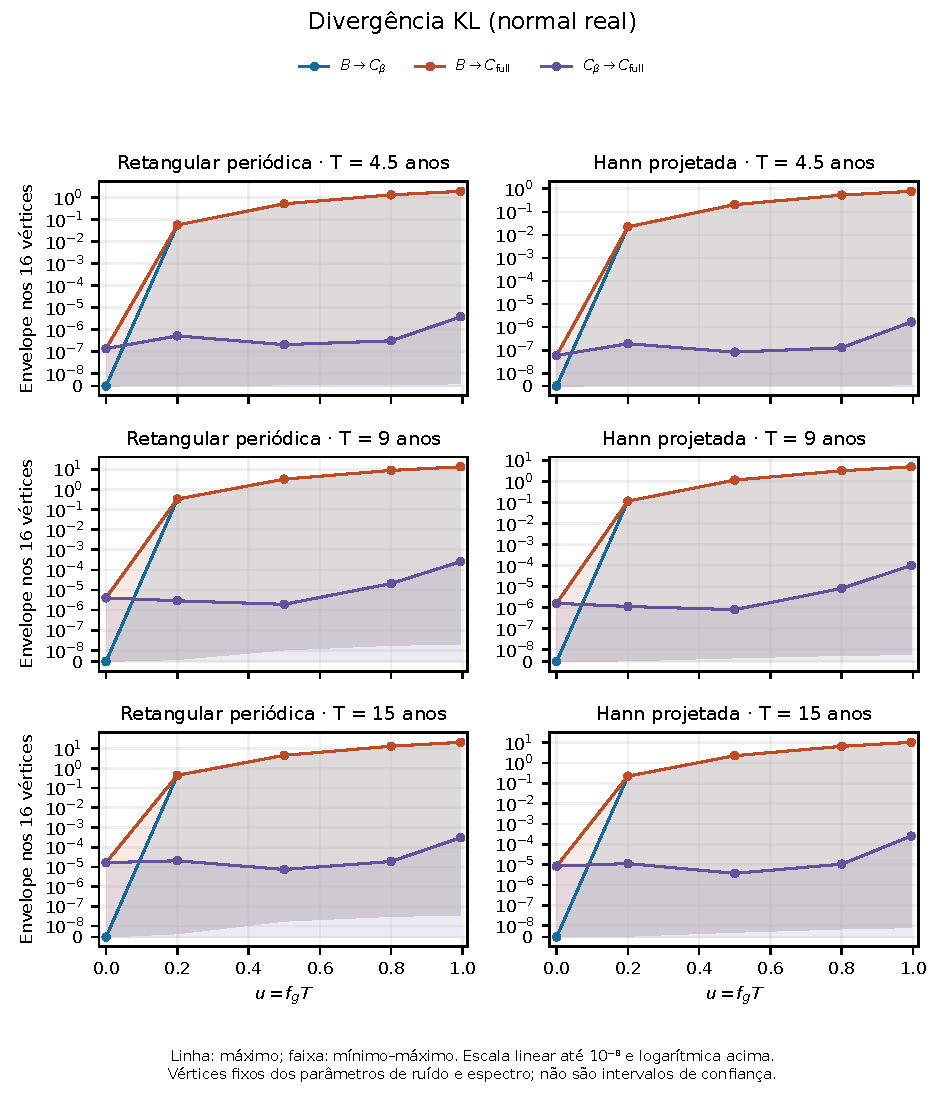
\includegraphics[width=0.94\textwidth,height=0.78\textheight,keepaspectratio]{../figures/compressao/mapa_janela/KL_p_to_q.pdf}
 \caption{Divergência $D_{\rm KL}[\mathcal N_p\Vert\mathcal N_q]$ dos momentos
 comprimidos. Linhas e faixas representam máximos e intervalos mínimo--máximo
 nos 16 vértices fixos, sem ponderação probabilística. Cada painel conserva
 sua duração e janela; o mapa termina em $u=0{,}995$.}
 \label{fig:comp-janela-kl}
\end{figure}

\begin{figure}[htbp]
 \centering
 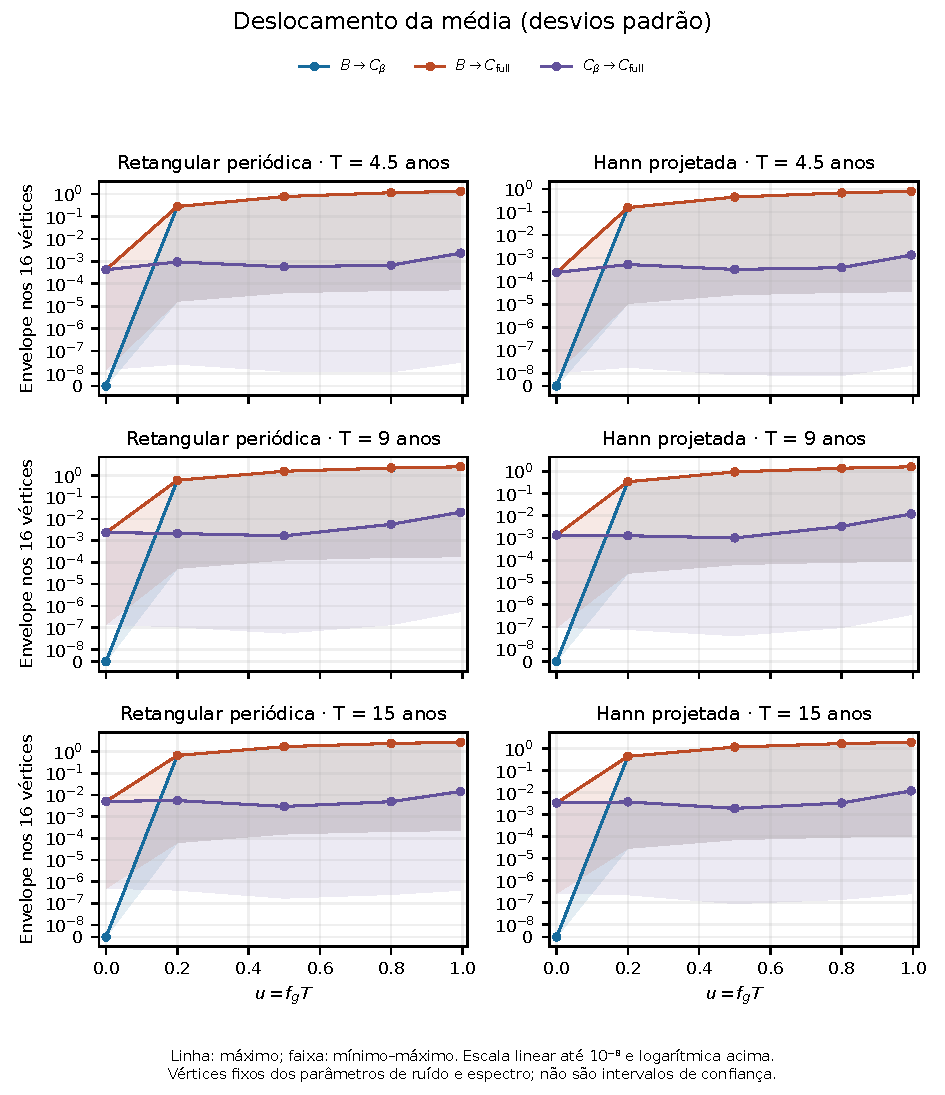
\includegraphics[width=0.94\textwidth,height=0.78\textheight,keepaspectratio]{../figures/compressao/mapa_janela/mean_shift_metric_p_squared.pdf}
 \caption{Deslocamento da média $d_\mu=\sqrt{\Delta\mu^T\Sigma_p^{-1}\Delta\mu}$
 no mesmo desenho da Figura~\ref{fig:comp-janela-kl}. A figura apresenta
 $d_\mu$, enquanto a Tabela~\ref{tab:comp-maximos-janela} apresenta seu
 quadrado.}
 \label{fig:comp-janela-media}
\end{figure}

\begin{figure}[htbp]
 \centering
 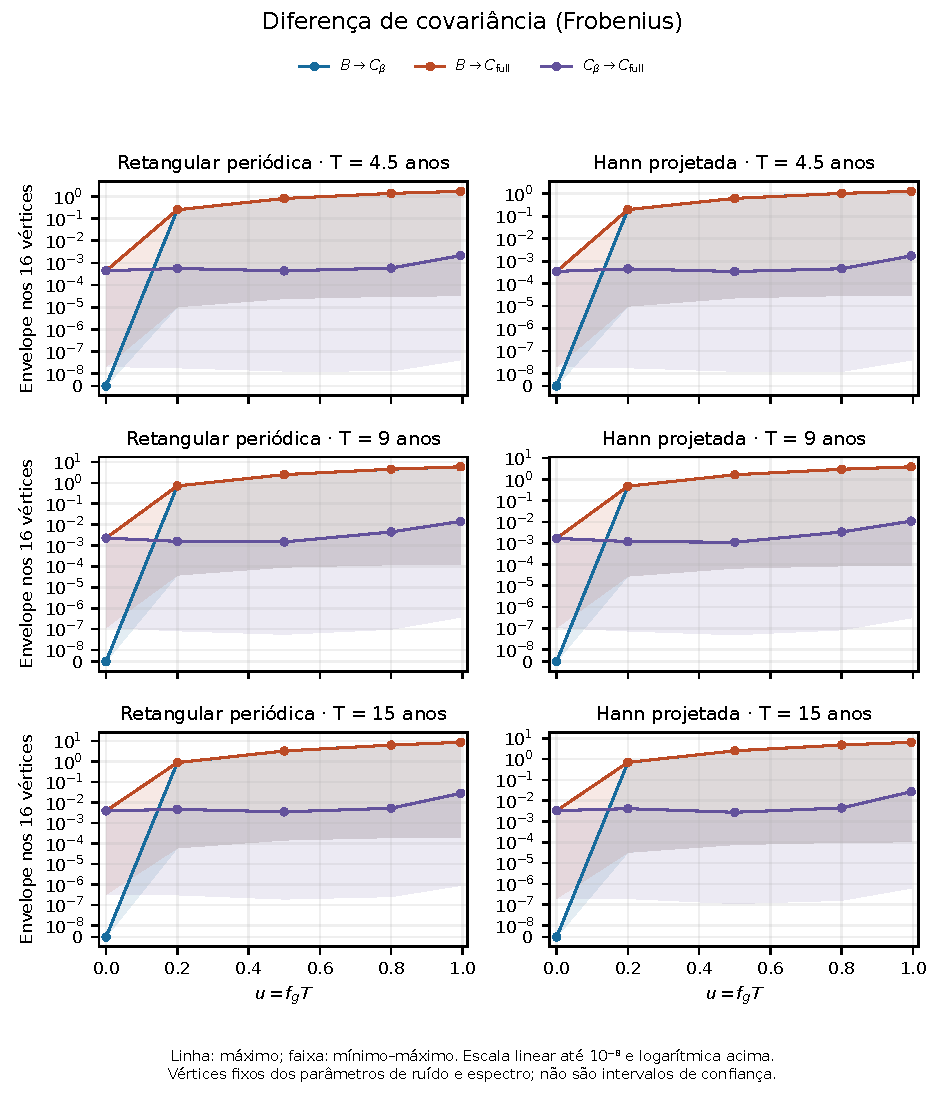
\includegraphics[width=0.94\textwidth,height=0.78\textheight,keepaspectratio]{../figures/compressao/mapa_janela/covariance_difference_metric_q.pdf}
 \caption{Discrepância $d_\Sigma$ da covariância, com branqueamento pela
 covariância da resposta $q$. Linhas e faixas têm o mesmo significado da
 Figura~\ref{fig:comp-janela-kl}. A operação conserva os blocos entre
 frequências introduzidos pela janela Hann projetada.}
 \label{fig:comp-janela-cov}
\end{figure}

\clearpage
\section{Resultados no limiar e na dispersão fraca}
\label{sec:comp-g2-fraca}

O mapa de duração e janela termina em $u=0{,}995$. Para examinar o limiar
sem extrapolar esse mapa, calculou-se uma grade adicional em
$u\in\{0;0{,}05;0{,}25;0{,}5;0{,}75;0{,}9;0{,}99;1\}$,
com $T=4{,}5$ anos, janela retangular e os mesmos 16 vértices dos parâmetros
auxiliares. As três respostas produzem 384 pares de média e covariância
distintos. Cada par foi avaliado em três resoluções harmônicas, separando
o refinamento da quadratura angular do aumento do corte multipolar.
Os valores em comum com o mapa anterior foram reutilizados por igualdade
exata do argumento e conferência da identidade dos arquivos.

Além dessa grade, três massas pequenas e três argumentos para diferenças
finitas da derivada exigiram uma extensão explícita do desenho: 67 novos
nós de frequência, 201 matrizes nas três resoluções e 12 avaliações
analíticas de derivadas. Os 13 processos sequenciais consumiram
95,54 segundos de CPU dos filhos, incluindo inicialização, com pico
de memória de aproximadamente 614 MiB (bytes do RSS convertidos por $2^{20}$). Esses custos são do mapa finito;
nenhuma posterior ou nova realização física foi gerada.

As discrepâncias máximas entre resoluções foram
$1{,}52\times10^{-12}$ nos momentos normalizados e
$1{,}92\times10^{-11}$ nas métricas gaussianas.
Uma reavaliação independente de 384 comparações na resolução fina,
por autovalores generalizados e fatorações de Cholesky, diferiu dos
resultados salvos em menos de $2{,}5\times10^{-15}$.
Essa verificação utiliza os momentos já calculados; não representa
uma segunda geração das respostas físicas.

\begin{table}[htbp]
\centering
\caption{Máximos no mapa adicional de oito massas e 16 vértices, em
$T=4{,}5$ anos e janela retangular. Cada coluna tem seu próprio máximo.
$d_\mu^2=\Delta\mu^T\Sigma_p^{-1}\Delta\mu$ e
$d_\Sigma=\|\Sigma_q^{-1/2}(\Sigma_p-\Sigma_q)\Sigma_q^{-1/2}\|_F$.
São métricas de distribuições normais construídas dos momentos.}
\label{tab:comp-g2-maximos}
\begin{tabular}{lrrr}
\toprule
Comparação $p\to q$ & $D_{\rm KL}(p\Vert q)$ & $d_\mu^2$ & $d_\Sigma$ \\
\midrule
$B\to C_\beta$ & 1,88683 & 1,73852 & 2,13177 \\
$B\to C_{\rm full}$ & 3,40909 & 2,29169 & 2,85437 \\
$C_\beta\to C_{\rm full}$ & 1,38410 & 1,00911 & 1,57542 \\
\bottomrule
\end{tabular}
\end{table}

Todos os máximos da tabela~\ref{tab:comp-g2-maximos} ocorrem no vértice
$(\log_{10}A_{\rm GW},\gamma,\log_{10}A_r,\log_{10}E)
=(-14,3,-17,-\log_{10}2)$.
Para $B\to C_\beta$, os máximos de KL e deslocamento quadrático da média
ocorrem em $u=0{,}99$; os demais máximos da tabela ocorrem em $u=1$.
O efeito de congelar as fases, isolado por $C_\beta\to C_{\rm full}$,
chega a $D_{\rm KL}=1{,}3841$ no limiar. Portanto, a pequena diferença
de fases encontrada no mapa restrito a $u\leq0{,}995$ não autoriza
concluir que essa diferença permanece pequena em todo o suporte.
Os valores dependem do vértice: em $u=1$, a KL desse contraste varia
de $2{,}77\times10^{-10}$ a $1{,}3841$.

A origem dessa dependência pode ser examinada sem uma integração angular
adicional. Em $\beta=0$, a expressão exata é
\begin{equation}
 \Gamma_{ab}(0,\boldsymbol y)
 =\frac{(1-e^{-iy_a})(1-e^{+iy_b})}{5}
 P_2(\hat p_a\cdot\hat p_b).
 \label{eq:comp-g2-limiar}
\end{equation}
Os fatores de fase permanecem na resposta. Repetir as fases do primeiro
canal nos demais canais modifica esses fatores, mesmo quando o argumento
dispersivo comum é zero. A expressão~\eqref{eq:comp-g2-limiar} concordou
com as matrizes numéricas dos quatro canais, nas três resoluções, com erro
absoluto máximo $1{,}31\times10^{-12}$.
Em $u=1$, o fator comum de $C_\beta$ e $C_{\rm full}$ é zero;
na resposta dispersiva B isso ocorre somente no primeiro canal.
Os demais canais de B conservam $\beta_k=\sqrt{1-k^{-2}}$.

\subsection{Verificação finita da primeira ordem}

A verificação utiliza a diferença $C_\beta-B$ e o sinal da
Eq.~\eqref{eq:comp-fraca}, com fases fixas e a primeira variação dos
momentos da Eq.~\eqref{eq:comp-g2-momentos-primeira-ordem}.
A derivada foi obtida analiticamente da
transferência regularizada e da contração dos coeficientes harmônicos.
Sua verificação por diferenças unilaterais de segunda ordem, com passos
$h=10^{-7}$ e $2h$, apresentou erro máximo normalizado
$2{,}93\times10^{-8}$, inferior à tolerância prospectiva $10^{-5}$.
As matrizes em $\beta=1$ obtidas nessa rota coincidem exatamente com
o cache utilizado. Não se exige positividade da matriz derivada.

Para $u=0{,}001;0{,}002;0{,}004$, a norma do resto de
$\Delta\Gamma$ cresce por fatores 15,9906 e 15,9623 quando $u$ dobra,
próximos da guia $2^4$. A razão entre a norma desse resto e a norma da
diferença completa é, respectivamente, 0,0206\%, 0,0824\% e 0,3295\%.
Nas covariâncias comprimidas, a razão relativa varia entre os vértices
de 0,0148\% a 0,0189\% na menor massa e de 0,2364\% a 0,3022\%
na maior. Duas razões consecutivas de restos de covariância não foram
reportadas porque o denominador ficou abaixo da guia de arredondamento
declarada, $1{,}42\times10^{-14}$. Essa guia operacional não é um
limite matemático do erro de arredondamento. Não se substituiu esse caso por zero nem se impôs razão 16.

A concordância apoia o mecanismo perturbativo no domínio finito testado.
Não fornece um limite uniforme para o resto ou autorização para usar a
expansão junto ao limiar. Também não se ajusta $C_{\rm full}-B$ a uma
lei sem termo constante em $u^2$: o congelamento das fases já pode produzir
uma diferença em $u=0$. Nenhuma dessas discrepâncias distribucionais,
isoladamente, é uma medida de viés posterior ou de cobertura de limites.

\begin{figure}[htbp]
 \centering
 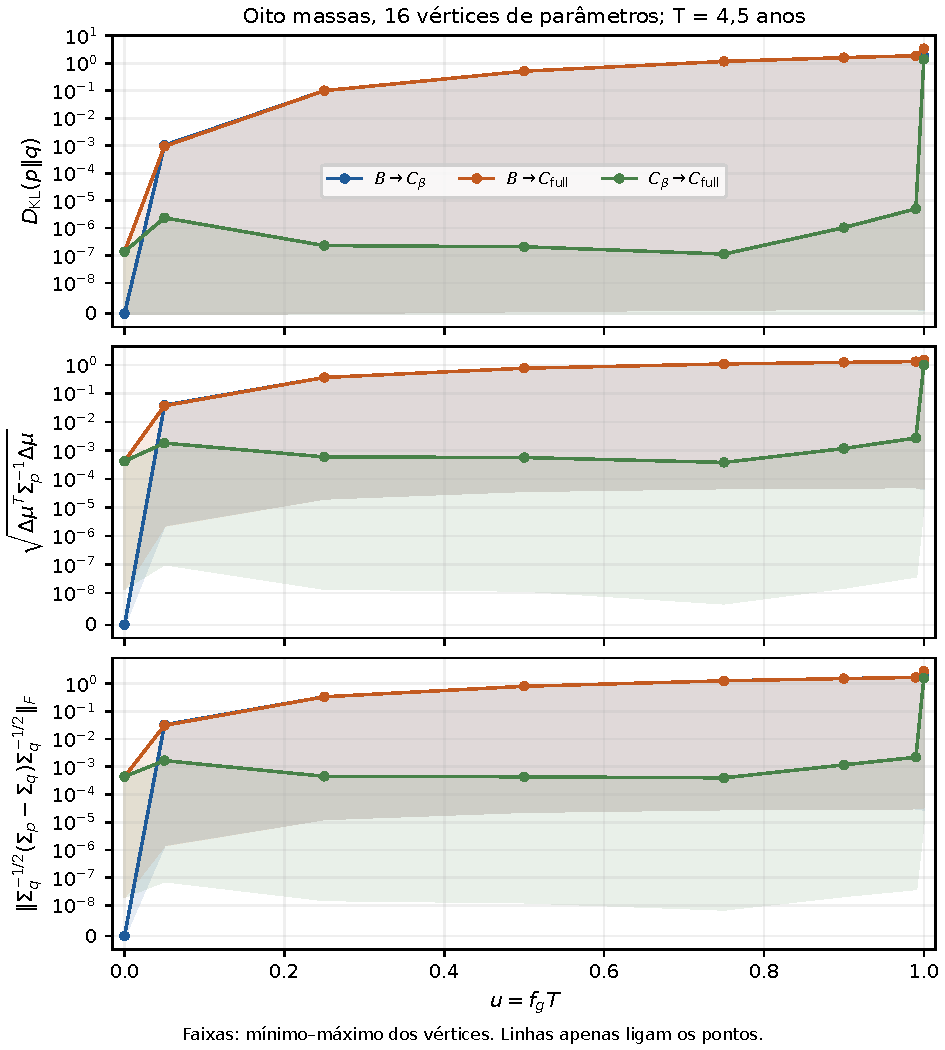
\includegraphics[width=0.96\textwidth,height=0.78\textheight,keepaspectratio]{../figures/compressao/g2_fraca/g2_momentos.pdf}
 \caption{Mapa adicional com oito valores de $u$, incluindo o limiar $u=1$,
 em $T=4{,}5$ anos e janela retangular. O painel central mostra $d_\mu$,
 enquanto o deslocamento da média é tabulado como $d_\mu^2$ na
 Tabela~\ref{tab:comp-g2-maximos}. As faixas são envelopes dos vértices;
 as linhas não substituem avaliações entre os pontos.}
 \label{fig:comp-g2}
\end{figure}

\begin{figure}[htbp]
 \centering
 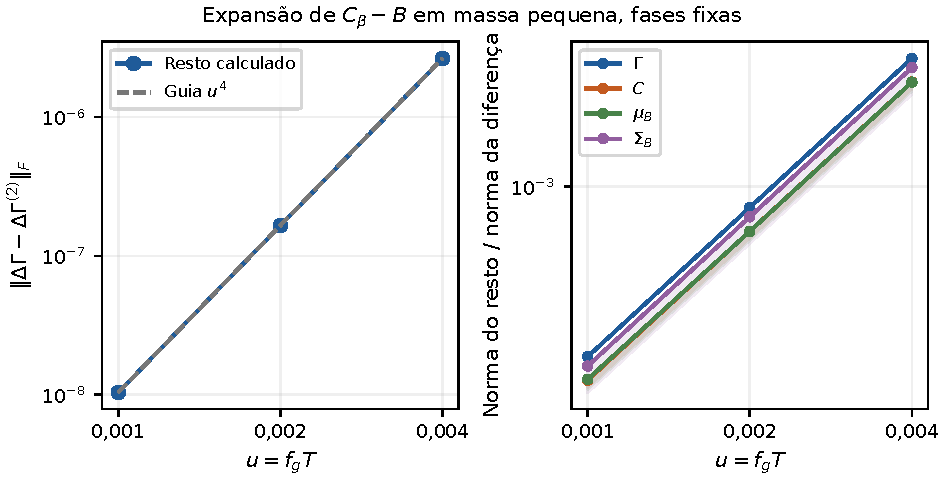
\includegraphics[width=\textwidth]{../figures/compressao/g2_fraca/expansao_fraca.pdf}
 \caption{Resto da expansão de $C_\beta-B$ até primeira ordem em $u^2$.
 À esquerda, norma de Frobenius do resto da resposta e guia proporcional
 a $u^4$, ancorada no primeiro ponto. À direita, norma do resto dividida
 pela norma da diferença completa, para a resposta, a covariância dos
 coeficientes e os dois momentos comprimidos. A guia não é um ajuste
 nem um limite uniforme do resto.}
 \label{fig:comp-fraca}
\end{figure}

\clearpage
\section{Comparações posteriores nas mesmas realizações}

% Texto opcional de integração: resultados publicados C07, apenas descrição.
\subsection{Descrição pareada das 500 realizações já publicadas}
\label{sec:comp-c07-descritivo}

A síntese publicada no capítulo~\ref{chap:validacao} permite descrever,
sem uma nova inferência, os contrastes A\_CN--A0\_CN, B\_CN--A\_CN e
B\_G--A\_G nos mesmos 500 dados. Nesta seção, a direção é sempre a
análise nova menos a anterior. Foram conferidos os 2.500 alvos, as 500
verdades originais e a identidade dos dados, prioris e arquivos publicados.
Todos os casos permanecem no resumo, inclusive aqueles com pendências
numéricas. A Tabela~\ref{tab:comp-descritivo500} mostra duas medidas de
posição das diferenças calculadas para a massa adimensional.

\begin{table}[htbp]
\centering\small
\caption{Descrição dos 500 valores pareados em unidades da largura da priori.
As médias e medianas não possuem aqui uma precisão horizontal certificada
dos quantis nem um intervalo de confiança associado.}
\label{tab:comp-descritivo500}
\begin{tabular}{lrrrr}
\toprule
Contraste & Média $\Delta Q_{95}(u)$ & Mediana & Média $\Delta W_{90}(u)$ & Mediana\\
\midrule
A\_CN$-$A0\_CN & 0,00130 & 0,00059 & $-0,00244$ & $-0,00007$\\
B\_CN$-$A\_CN & 0,00540 & $-0,00127$ & 0,01147 & 0,00213\\
B\_G$-$A\_G & 0,00477 & $-0,00061$ & 0,00652 & 0,00137\\
\bottomrule
\end{tabular}
\end{table}

As diferenças de quantis e de larguras são computadas por dado antes de
qualquer média ou mediana. Em dois contrastes, a média e a mediana de
$\Delta Q_{95}(u)$ têm sinais distintos. Esse fato limita a interpretação
da média isolada; não determina a direção de um deslocamento para cada
realização. A descrição completa retém os 20 quantis e as cinco larguras
centrais de 90\%, com as guardas por função preservadas em arquivos.

Os bins fixos $u\in[0;0{,}5),[0{,}5;0{,}9),[0{,}9;1]$ contêm
243, 208 e 49 dados; os bins $\gamma\in[3;4{,}25),[4{,}25;5{,}5]$
contêm 233 e 267 dados. As subdivisões se baseiam nas verdades e não
selecionam realizações pelo resultado das guardas. Percentis entre os casos,
quando apresentados nos arquivos, descrevem essa distribuição empírica;
não são intervalos de confiança da média. Pequenas diferenças ou
proximidade entre curvas não são convertidas em decisões de equivalência,
materialidade ou viés populacional. A análise inferencial pareada, com
brackets e incerteza explicitamente avaliados, permanece separada.

\begin{figure}[htbp]
 \centering
 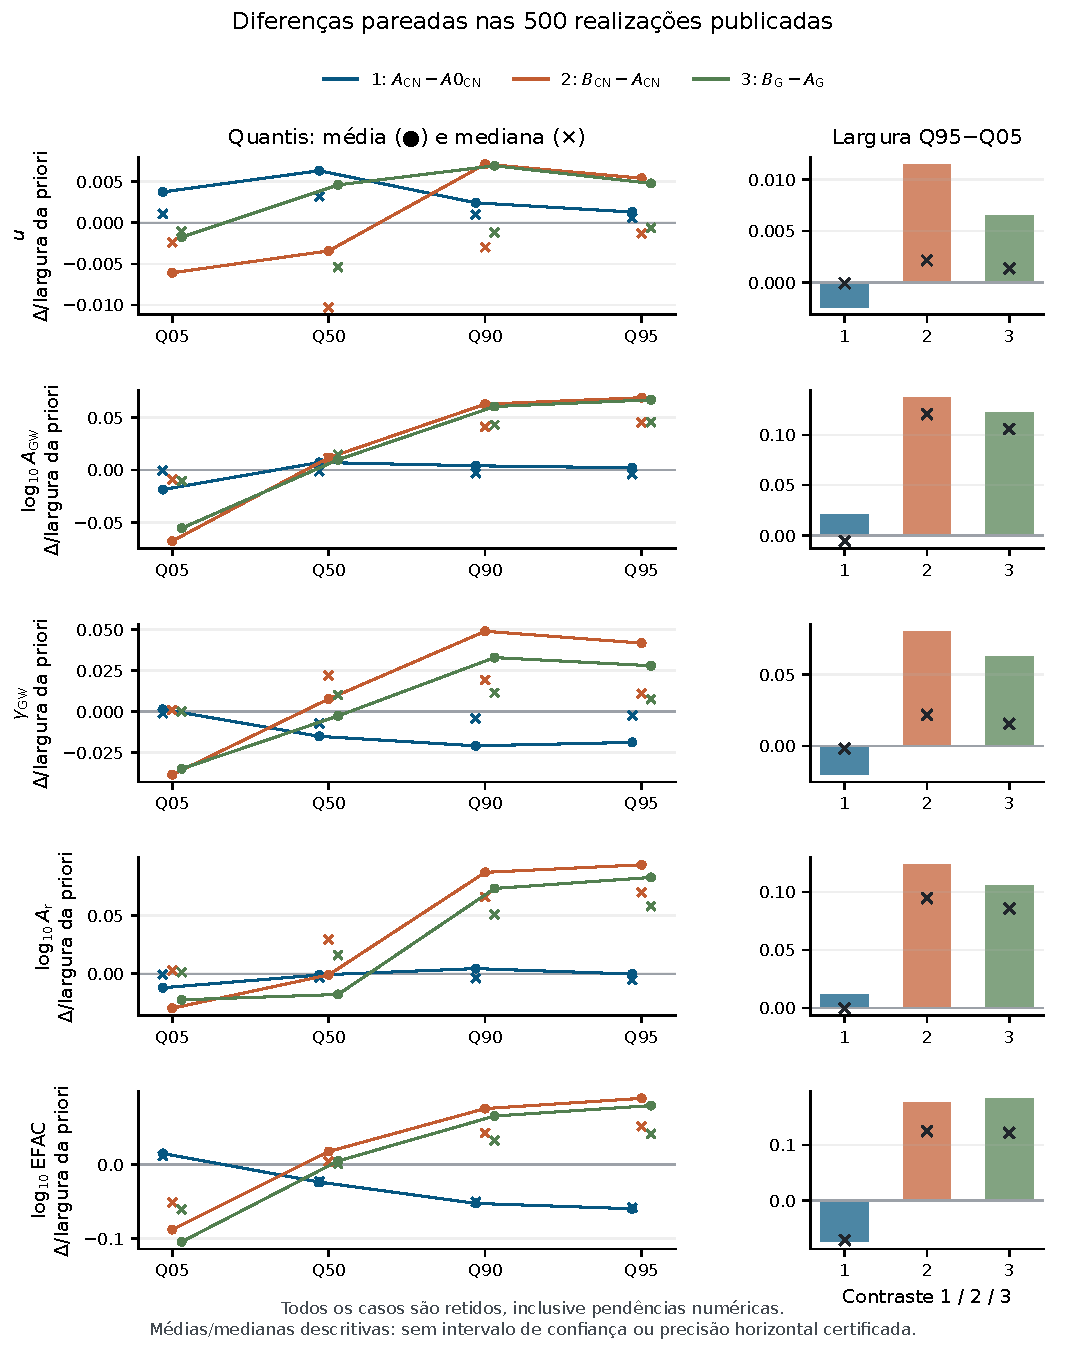
\includegraphics[width=\textwidth,height=.80\textheight,keepaspectratio]{../figures/compressao/c07_descritivo/paired_quantiles_widths.pdf}
 \caption{Médias e medianas descritivas das diferenças pareadas nos 500 dados
 publicados. A largura central é $W_{90}=Q_{95}-Q_{05}$. Todos os casos são
 retidos; a figura não contém barras de erro numérico ou intervalos de confiança.}
 \label{fig:comp-c07-pares}
\end{figure}

\begin{figure}[htbp]
 \centering
 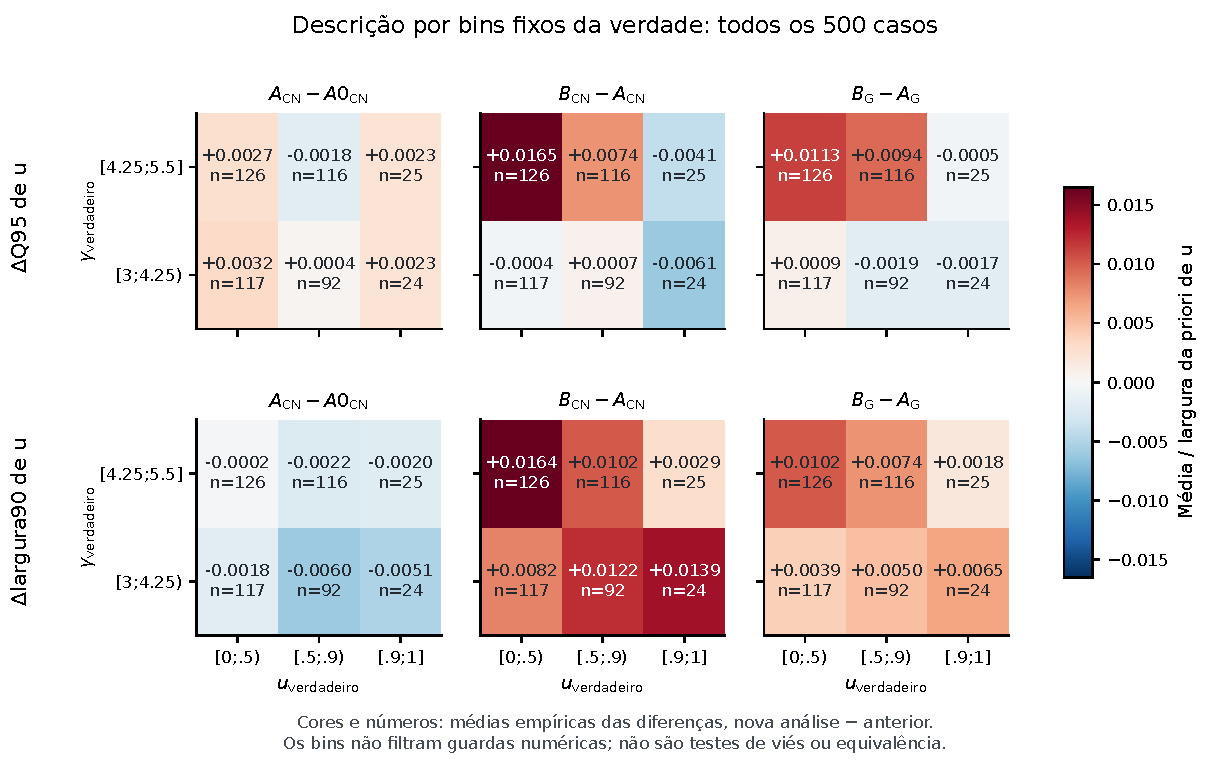
\includegraphics[width=\textwidth]{../figures/compressao/c07_descritivo/paired_mass_bins.pdf}
 \caption{Médias descritivas de $\Delta Q_{95}(u)$ e $\Delta W_{90}(u)$
 nos bins fixos da verdade. Cada célula informa seu número de dados;
 as pendências numéricas permanecem no denominador. As cores não expressam
 significância estatística nem equivalência entre as análises.}
 \label{fig:comp-c07-bins}
\end{figure}

\clearpage
\subsection{Protocolo pareado e separação dos erros}
\label{sec:comp-pareado-protocolo}

A comparação principal reúne nove análises nos mesmos 32 dados: os cinco
modelos do estudo de calibração e as variantes $C_\beta$ e $C_{\rm full}$,
aplicadas aos dados CN e G. Vinte e quatro IDs foram sorteados sem reposição
da campanha original, com semente previamente fixada; oito testes de
fronteira foram selecionados separadamente. Somente os 24 primeiros entram
na síntese piloto da média. Os oito testes de fronteira permanecem visíveis
como casos individuais, sem representar amostragem da priori nem aumentar
o tamanho amostral dessa média.

Para cada variante C foram concluídos 64 alvos, após oito controles de
engenharia. A produção segue o treino independente e as quatro réplicas IID
do Capítulo~\ref{chap:validacao}, com 16.384 e 65.536 amostras por réplica
nos níveis LOW e HIGH. Nenhuma proposta foi selecionada pela verdade do
parâmetro. O diagnóstico geral de pesos ficou pendente em um alvo de
$C_\beta$ e em cinco de $C_{\rm full}$; todos os alvos e seus diagnósticos
foram preservados. Esse diagnóstico geral não substitui a avaliação de
precisão dos quantis apresentada nesta seção.

Os cinco modelos de referência contribuem com 160 conjuntos HIGH. Sua reprodução
utilizou as propostas, sementes, estados inicial e final do gerador e
receitas originais. Os arquivos reproduzidos foram comparados pelo SHA-256
com os arquivos originais antes da retirada dos dados brutos. Essa
reprodução acrescenta diagnósticos aos mesmos cálculos, sem constituir
novas realizações independentes para a calibração. A análise conserva os
quantis de probabilidades 0,05, 0,50, 0,90 e 0,95 dos cinco parâmetros,
totalizando 5.760 quantis nos 288 pares modelo--dado.

O alvo primário é a mudança do limite $U_{95}$ de $u$. Adotou-se previamente
uma escala de interesse de 0,01 da largura da priori. Os sete contrastes,
sempre análise nova menos anterior, são A\_CN$-$A0\_CN, B\_CN$-$A\_CN,
B\_G$-$A\_G, $C_{\beta,\rm CN}-$B\_CN, $C_{\beta,\rm G}-$B\_G,
$C_{{\rm full},\rm CN}-C_{\beta,\rm CN}$ e
$C_{{\rm full},\rm G}-C_{\beta,\rm G}$. Os outros 19 quantis e as cinco
larguras $Q_{95}-Q_{05}$ são produtos descritivos secundários.

A precisão horizontal de um quantil não é deduzida dividindo o erro da
CDF por uma densidade estimada. Os cortes foram escolhidos exclusivamente
no LOW, antes de examinar o HIGH. Para cada quantil são usados os extremos
0 e 1 e até 21 cortes em torno da posição LOW, com deslocamentos fixos de
0,0005 até 0,256 em coordenadas da priori. A CDF HIGH em cada corte usa
MCSE da influência SNIS e a dispersão entre réplicas independentes;
ESS não é usado como tamanho de uma amostra binomial.

As bandas de CDF reservam famílias de 6.624 comparações para $U_{95}(u)$ e
125.856 para os demais quantis, com $\alpha=0,025$ em cada família. São
mantidas as verificações de peso, saturação e estabilidade da normalização
entre LOW e HIGH e entre réplicas. Uma falha comum ou ausência de uma
avaliação operacional da resposta produz o intervalo numérico $[0,1]$,
que continua na síntese. A diferença de dois intervalos é propagada como
\begin{equation}
 \bigl[\ell_{\rm novo}-h_{\rm anterior},\;
  h_{\rm novo}-\ell_{\rm anterior}\bigr].
\end{equation}
Um intervalo inteiramente acima de 0,01 ou abaixo de $-0,01$ identifica
um deslocamento material resolvido no caso. Um intervalo contido em
$[-0,01;0,01]$ indica compatibilidade operacional nessa realização;
os demais permanecem inconclusivos.

Para as sete médias dos 24 IDs usa-se bootstrap pareado por dado, com
10.000 reamostragens e semente 808110601. O mesmo sorteio de IDs é usado
nos sete contrastes. Publicam-se os percentis de caudas $0,05/(2\times7)$
das estimativas pontuais e a envoltória correspondente dos limites
numéricos inferiores e superiores. Essa construção é uma aproximação
operacional que incorpora a variação entre dados e a incerteza dos
quantis. Não constitui garantia conjunta de cobertura de 95\%, teste de
equivalência populacional ou calibração SBC de 32 dados. Os bins de massa
e índice espectral seguem os limites já fixados na descrição dos 500
casos, sempre com seus números efetivos de observações.

\subsection{Controles finitos da resposta no domínio posterior}
\label{sec:comp-controles-finitos}

A margem operacional de 0,002 na CDF foi examinada em uma malha fixada
antes das avaliações físicas. Os 17 valores de $u$ combinam nove âncoras
uniformes com oito posições obtidas exclusivamente dos quantis LOW.
Para cada par modelo--dado, quatro réplicas de 128 pontos dos quatro
parâmetros auxiliares usam a marginal da proposta LOW correspondente.
Os 17 valores de massa compartilham o mesmo ponto auxiliar: existem
512 grupos IID, e não 8.704 observações independentes. A integração em
$u$ usa pesos trapezoidais positivos. As comparações emparelham a
implementação nativa com a referência harmônica e refinam separadamente
as duas resoluções harmônicas, a malha de massa e o número de grupos.

Para cada corte, a regra prospectiva soma o módulo da diferença de CDF,
sua MCSE multiplicada pelo quantil normal com ajuste para multiplicidade,
e as mudanças dessa diferença sob os dois refinamentos. O total deve
ser menor ou igual a 0,002. Também se exige peso máximo por grupo de
0,1, mudança pareada por deleção de no máximo 0,0005, suporte finito e
justificativa algébrica quando a MCSE é exatamente zero. A família
principal possui limite de 397.440 comparações; as 36 vinculações dos
quatro casos de engenharia usam outra família, de 49.680. Estas últimas
reutilizam os mesmos valores físicos com seus cortes próprios e não
constituem novas réplicas independentes.

Foram preservadas 288 nuvens, 324 análises vinculadas e 416.856
comparações de cortes. Quatro nuvens ficaram inconclusivas por saturação
da transformação sem recorte: A0\_CN/409, B\_G/489,
$C_{\beta,\rm CN}$/48 e $C_{\beta,\rm G}$/359. Não se sorteou uma
substituição. Entre os valores finitos avaliados, a discrepância máxima
de logL entre as resoluções harmônicas foi $9{,}54\times10^{-8}$;
entre a implementação nativa e a referência harmônica,
$8{,}88\times10^{-6}$; e nas sondas SciPy independentes,
$1{,}60\times10^{-11}$. Esses máximos respeitam as tolerâncias adotadas
nos pontos examinados, sem controlar todo o domínio contínuo.

\begin{table}[htbp]
\centering\small
\caption{Resultado dos controles finitos por análise, com 32 dados
retidos em cada linha. Aprovação significa cumprir as regras operacionais
nos cortes avaliados; não certifica o erro de toda a CDF posterior.}
\label{tab:comp-controles-finitos}
\begin{tabular}{lrr}
\toprule
Análise & Regras satisfeitas & Inconclusivos\\
\midrule
A0\_CN & 1 & 31\\
A\_CN & 0 & 32\\
B\_CN & 1 & 31\\
A\_G & 3 & 29\\
B\_G & 0 & 32\\
$C_{\beta,\rm CN}$ & 4 & 28\\
$C_{\beta,\rm G}$ & 3 & 29\\
$C_{{\rm full},\rm CN}$ & 32 & 0\\
$C_{{\rm full},\rm G}$ & 32 & 0\\
\midrule
Total & 76 & 212\\
\bottomrule
\end{tabular}
\end{table}

As falhas incluem MCSE nula sem comprovação da identidade requerida;
esse estado não demonstra uma discrepância física grande. Nos casos
de suporte não resolvido, os indicadores preservam explicitamente a
ausência de uma avaliação válida. A maior mudança absoluta da CDF da
medida de controle ao refinar a malha de massa foi 0,1888. Portanto, a
estabilidade da \emph{diferença entre implementações} não deve ser
interpretada como precisão absoluta dessa quadratura ou como limite
uniforme do erro posterior. O resultado é um diagnóstico finito e
operacional, com alcance menor que uma certificação de quantis.

A análise compacta original atingiu o teto de CPU depois que terminaram
as avaliações físicas. Seu estado de falha e os 143 relatórios completos
foram preservados. Uma continuação exclusivamente estatística calculou
os 181 relatórios faltantes, sem novas verossimilhanças, ORFs ou amostras.
Os custos externos foram 597,413 s de CPU na execução original e
56,304 s na continuação, totalizando 653,717 s sob orçamentos separados.
Foram cobrados 9.892.288 valores de verossimilhança dos 10.031.616
reservados; a diferença decorre das interrupções locais por saturação.

Os diagnósticos originais dos 5.760 quantis continuam imutáveis.
Uma avaliação suplementar aplica os controles às estatísticas de CDF
já arquivadas, conservando cortes, MCSE, pesos e demais regras. Produziu
1.460 intervalos operacionais e manteve 4.300 intervalos inconclusivos
$[0,1]$. Um intervalo operacional ainda pode ser largo para a escala
de interesse de 0,01; sua existência não implica equivalência entre
duas análises. Nenhum caso inconclusivo é excluído das comparações.

\subsection{Resultado da comparação pareada dos limites}
\label{sec:comp-pareado-resultado}

Os sete contrastes mantiveram os 32 dados e todos os intervalos numéricos.
Nenhuma das 224 comparações individuais de $U_{95}(u)$ resolveu
compatibilidade ou diferença material na escala de 0,01. As sete médias
do piloto representativo também permaneceram inconclusivas depois de
propagar os intervalos numéricos. Esse resultado identifica uma
limitação de resolução da campanha; não demonstra que os efeitos sejam
nulos nem que a aproximação de frequência de referência seja adequada.

\begin{table}[htbp]
\centering\small
\caption{Média de $\Delta U_{95}(u)$ nos 24 dados representativos e
envoltórias bootstrap. Valores em unidades da largura da priori.
A coluna pontual ignora a incerteza horizontal dos quantis; a última
propaga os intervalos operacionais, inclusive os inconclusivos.}
\label{tab:comp-pareado-medias}
\begin{tabular}{lrrr}
\toprule
Contraste & Média pontual & Bootstrap pontual & Com erro numérico\\
\midrule
A\_CN$-$A0\_CN & 0,00655 & $[0,00089;0,01494]$ & $[-1;1]$\\
B\_CN$-$A\_CN & $-0,00411$ & $[-0,00792;-0,00050]$ & $[-1;1]$\\
B\_G$-$A\_G & 0,00642 & $[-0,00145;0,02137]$ & $[-1;1]$\\
$C_{\beta,\rm CN}-$B\_CN & $-0,00005$ & $[-0,00112;0,00075]$ & $[-1;1]$\\
$C_{\beta,\rm G}-$B\_G & $-0,00053$ & $[-0,00320;0,00086]$ & $[-1;1]$\\
$C_{{\rm full},\rm CN}-C_{\beta,\rm CN}$ & 0,00007 & $[-0,00029;0,00043]$ & $[-0,05387;0,96174]$\\
$C_{{\rm full},\rm G}-C_{\beta,\rm G}$ & 0,00010 & $[-0,00024;0,00045]$ & $[-0,36607;0,97144]$\\
\bottomrule
\end{tabular}
\end{table}

As pequenas médias pontuais de B--C não autorizam uma conclusão de
equivalência. Do mesmo modo, a envoltória do bootstrap pontual de
B\_CN$-$A\_CN não é evidência suficiente de uma diferença resolvida:
ela omite justamente a componente numérica que torna o resultado
inconclusivo. Os oito casos de fronteira possuem suas próprias tabelas
e figuras individuais e não entram no bootstrap dos 24 casos.
Nenhum ponto original ficou fora de seu intervalo suplementar.

\begin{figure}[htbp]
\centering
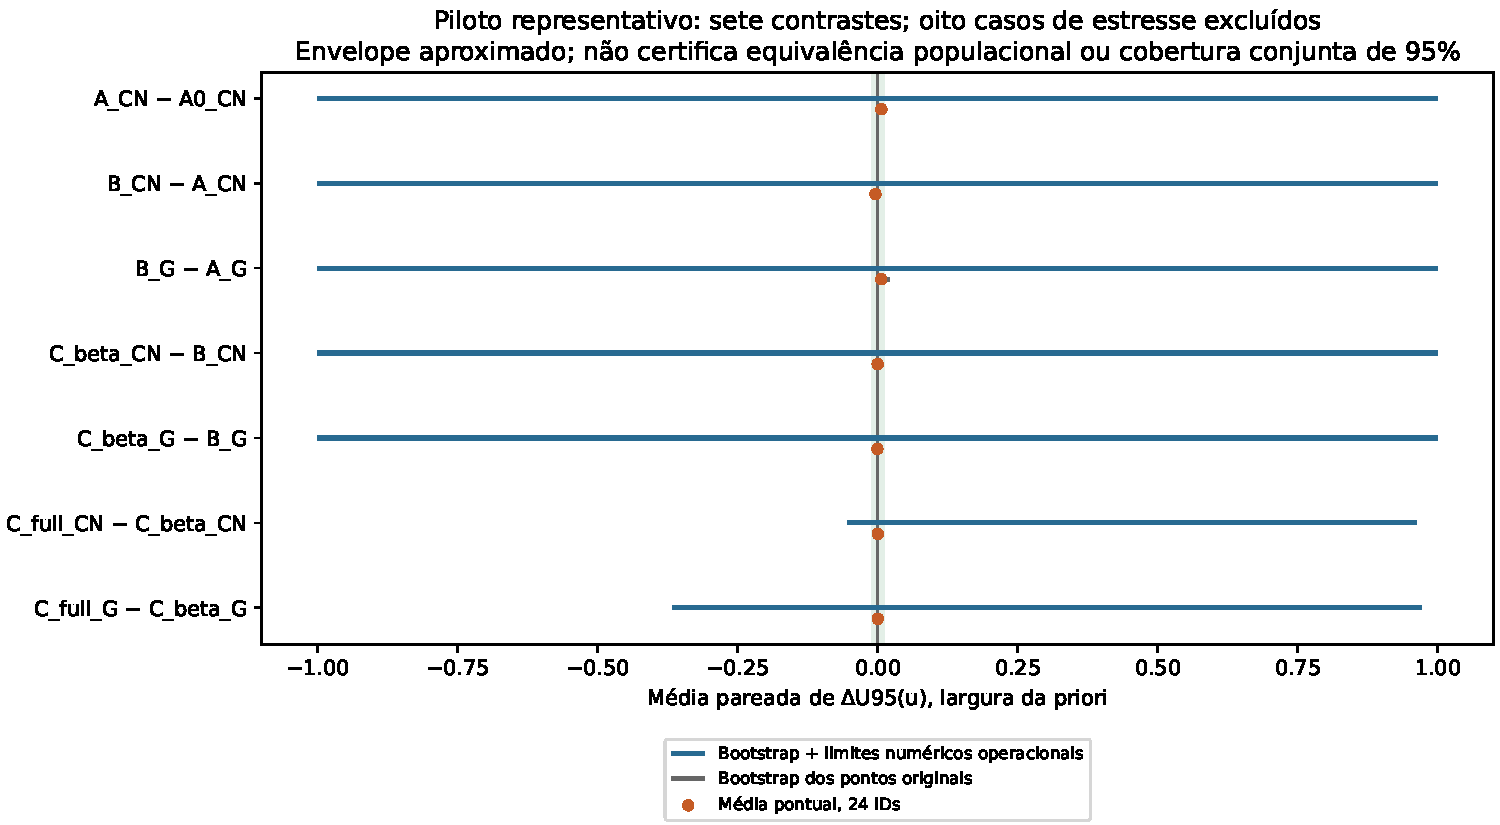
\includegraphics[width=\textwidth]{../figures/compressao/pareado32/u95_representative_mean.pdf}
\caption{Comparação das sete médias pareadas no piloto representativo.
As faixas azuis propagam as pendências numéricas; as faixas cinzas usam
somente os pontos originais. A faixa verde indica a escala prospectiva
$[-0,01;0,01]$. A resolução dos intervalos, e não a proximidade visual
dos pontos a zero, governa a classificação.}
\label{fig:comp-pareado-medias}
\end{figure}

Os arquivos públicos preservam 4.480 diferenças de quantis e 1.120
diferenças de larguras centrais, além dos 10.000 sorteios bootstrap das
médias já calculadas. As subdivisões em massa e índice espectral
conservam suas contagens e não produzem estimativas de cobertura
condicional. Uma recomposição independente verificou exatamente os
contrastes, a propagação de intervalos e larguras e os percentis
calculados a partir das médias bootstrap arquivadas. A conclusão
inferencial deste estudo é, portanto, delimitada: foram medidos os
deslocamentos pontuais, mas sua resolução operacional não sustenta um
domínio de equivalência de limites de massa na coorte examinada.

\subsection{Forma posterior em quatro controles normais}
\label{sec:comp-KL-posterior}

Nos quatro IDs fixados para engenharia, avaliou-se também a divergência
entre as posteriores A\_G e B\_G nos mesmos dados normais. A estimativa usa
\begin{equation}
 D_{\rm KL}\!\left[p_A(\theta\mid A)\,\Vert\,p_B(\theta\mid B)\right]
 =\mathbb E_{p_A}[\log L_A-\log L_B]+\log Z_B-\log Z_A .
 \label{eq:comp-KL-posterior}
\end{equation}
Os termos de normalização completam a razão de densidades posteriores
no mesmo espaço de parâmetros. Sua combinação na expressão não é um
fator de Bayes entre A e B, que pertencem a espaços de dados distintos.
A expectativa de logL de B foi calculada nos mesmos sorteios HIGH de A,
com 1.048.576 avaliações adicionais. As estimativas de $Z_B$ usam as
réplicas independentes já reproduzidas de B.

\begin{table}[htbp]
\centering\small
\caption{Divergência posterior A\_G para B\_G nos quatro dados de
engenharia. MCSE assintótica, em nats; não é erro entre realizações
nem certificação determinística do cálculo.}
\label{tab:comp-KL-posterior}
\begin{tabular}{rrr}
\toprule
ID & $D_{\rm KL}$ estimada & MCSE\\
\midrule
25 & 0,63803 & 0,00250\\
26 & 1,47700 & 0,00358\\
44 & 3,49123 & 0,00377\\
48 & 0,58490 & 0,00259\\
\bottomrule
\end{tabular}
\end{table}

A propagação retém a covariância entre a expectativa ponderada e
$\log Z_A$, além da contribuição independente de $\log Z_B$.
Primeiros e segundos momentos conjuntos também foram arquivados para
reconstruir as covariâncias posteriores. Uma auditoria independente
recompôs essas quantidades a partir das estatísticas suficientes;
os quatro pares satisfizeram seus diagnósticos de peso e suporte.
As divergências não foram truncadas em zero nem usadas para escolher
os IDs. O resultado quantifica diferenças de forma em quatro dados
específicos, sem estimar uma ordenação populacional de perdas ou
substituir a análise dos limites de massa.

\section{Alcance dos resultados concluídos}

Os mapas localizam discrepâncias entre respostas e identificam dois
mecanismos: a diferença de dispersão entre canais já aparece em ordem
$u^2$, e o congelamento das fases pode se tornar relevante junto ao limiar.
A janela Hann projetada exige covariâncias entre frequências. Essas
conclusões dizem respeito ao setor tensorial e ao experimento idealizado
de 12 pulsares e quatro modos descrito neste trabalho.

As métricas normais aqui calculadas são funções dos momentos em parâmetros
fixos. Elas não medem, por si, deslocamento de quantis posteriores,
calibração ou evidência bayesiana. A demonstração de processamento de dados
trata de experimentos corretamente especificados; o mapa de $B$ contra
$C_\beta$ ou $C_{\rm full}$ examina também mudança do modelo.
As comparações inferenciais pareadas foram concluídas com todos os
casos retidos. A resolução numérica não permitiu classificar os efeitos
na escala prospectiva de 0,01; assim, o estudo não estabelece que a
aproximação preserve os limites de massa nem uma direção universal de
viés. Melhorar a resolução das CDFs, especialmente nos casos de MCSE
nula sem prova suficiente, permanece uma extensão metodológica.
Os estudos seguintes de robustez tratam questões próprias e não
transformam essa pendência em uma validação já obtida.
